\documentclass[runningheads]{llncs}

\usepackage[hidelinks]{hyperref}

\usepackage{subcaption}
\usepackage{tikz}
\usepackage{url}
\usetikzlibrary{positioning}
\usetikzlibrary{scopes}
\usetikzlibrary{fit}
\usetikzlibrary{arrows.meta}
\usetikzlibrary{shapes}

\newcommand{\dummyfigsmall}[1]{
  \centering
  \fbox{
    \begin{minipage}[c][0.1\textheight][c]{0.5\textwidth}
      \centering{#1}
    \end{minipage}
  }
}

\newcommand{\dummyfiglarge}[1]{
  \centering
  \fbox{
    \begin{minipage}[c][0.35\textheight][c]{0.5\textwidth}
      \centering{#1}
    \end{minipage}
  }
}

\begin{document}

\title{Sterling: A Web-based Visualizer\\ for Relational Modeling Languages}
\author{Tristan Dyer \inst{1} \and John Baugh \inst{2}}
\authorrunning{Dyer and Baugh}

\institute{Brown University \and North Carolina State University}

\authorrunning{Dyer and Baugh}

\maketitle

\begin{abstract}
We introduce Sterling, a web-based visualization tool that provides interactive views of relational models and allows users to create custom visualizations using modern JavaScript libraries like D3 and Cytoscape.
We outline its design goals and architecture, and describe custom visualizations developed with Sterling that enable verification studies of scientific software used in production.
While development is driven primarily by the Alloy community, other relational modeling languages are accommodated by Sterling's data agnostic architecture.
\end{abstract}

% \begin{abstract}
% We introduce Sterling, a web-based visualization tool for Alloy that provides enhanced views of relational models and amends some of the recognized shortcomings of its approach to graph layout.
% A scripting view gives users the ability to create custom visualizations using modern JavaScript libraries such as D3 and Cytoscape without sacrificing the immediate visual feedback provided by Alloy. This enables users to more easily develop and understand relational models with characteristics beyond those that are purely topological, where space and position matter, for instance.
% We demonstrate effective use of the scripting view by presenting custom visualizations developed to enable verification studies of production scientific software.
% While development is driven primarily by the Alloy community, other relational logic and model finding tools can also be accommodated in its model-view architecture, which uses a mediator pattern to keep the approach data agnostic. One such tool, Forge, a relational language and tool built for teaching introductory formal methods as Brown University, employs Sterling as its visualizer.
% \end{abstract}

% \begin{abstract}
% We introduce Sterling, a web-based visualization tool for Alloy that provides enhanced versions of existing Alloy visualizations and introduces new capabilities to address shortcomings of the visual abstractions typically used to display instances of relational models.
% While development is driven primarily by the needs of the Alloy community, other relational logic and model finding tools are accommodated by its model-view architecture, which uses a mediator pattern to keep the approach data agnostic.
% We describe our design goals and demonstrate effective use of Sterling by presenting custom visualizations of models with inherently spatial characteristics.
% \end{abstract}

\keywords{Alloy \and Sterling \and Formal Methods \and Visualization}

\section{Introduction}
\label{introduction}

Model finding tools like Alloy enable a lightweight approach to design and reasoning about complex software systems. Such tools provide push-button analysis for both checking assertions within bounded scopes, and for generating instances that satisfy a property of interest. An attractive feature of Alloy is the immediate feedback provided by visualizations, allowing users to inspect instances and counterexamples in order to identify design problems. The ability to communicate visual information \emph{intuitively} therefore plays a key role in determining the effectiveness of interactions with the user~\cite{gammaitoni2014}.

The Alloy Analyzer includes a visualizer that can display an instance as a directed graph in which nodes represent atoms and edges represent tuples of relations.
To help users better understand an instance, basic properties of the graph such as color and shape can be customized, and graph nodes can repositioned manually to achieve a clearer layout.
Additionally, the graph view supports ``projection,'' a feature most commonly used with models of dynamic systems. 
When an instance of such a model is projected over time, the user is able to step through snapshots of individual states in sequence.

Despite these capabilities, some instances can be difficult to interpret as models grow in size and complexity.
Some well-known issues, for instance, include the inability to drag nodes out of the rows into which they are initially laid out~\cite{couto2018,macedo2019}.
In addition, the graph layout is recalculated any time a new instance is generated or the projection is changed, so the user is forced to reinterpret the entire graph if, for example, they are stepping through the state atoms in sequence~\cite{couto2018,misue1995,zaman2013}.
Various approaches have been proposed to address these and other issues, either by extending the existing visualizer~\cite{zaman2013} or by introducing new tools~\cite{couto2018,macedo2019,gammaitoni2014}.
% While various approaches have been proposed to address these and other issues, either by extending the existing visualizer~\cite{zaman2013} or by introducing new tools~\cite{couto2018,macedo2019,gammaitoni2014}, our own experience using Alloy in the field of scientific computing has highlighted the need for an approach that facilitates the clear expression of \emph{spatial} relationships---not just topological ones---and to \emph{consistency} in those relationships when dynamic updates occur, as they do in problems with time-varying state.
%
% {\color{red}The transition here needs to be that our prior studies
%   motivate what we're doing now.  Otherwise the reader will think
%   we're about to describe other ``prior'' visualization work instead
%   of work that motivates better visualization.  E.g., something like
%   ... Beyond these limitations, our own work has demonstrated the need
%   for improved visualization and the ability to customize ... no
%   ``print'' statements, and need to interpret rich state.}
%
Our own experiences with Alloy in the field of scientific computing have highlighted the need for better visualization approaches in general, and for an interface that can also depict \emph{spatial} relationships---not just topological ones---while maintaining \emph{consistency} in those relationships when dynamic updates occur, as they do in problems with time-varying state.

% This work, which we describe below, has additionally demonstrated the need for an approach that facilitates the expression of rich state and enables users to choose an appropriate visual abstraction without being restricted by the design and implementation choices of the visualizer.
For instance, in one such study, Baugh and Altuntas~\cite{baugh-scp-2018} use Alloy to explore implementation choices and ensure soundness of an extension made to a large-scale storm surge application used in production.
To be physically meaningful, models representing finite element meshes---which can be thought of as a triangulation of a surface---are constrained to include only those that have a planar embedding.
Working with relational depictions alone means ``untangling'' each instance as it occurs, leading to the study's conclusion that ``more than any extension to Alloy, what would have benefited our study most is a tool capable of automatically producing planar embeddings of meshes from Alloy instances, which proved to be tedious to do by hand.''
In a subsequent study~\cite{dyer2019} with Alloy, our group performs bounded verification of sparse matrix formats, which use array indirection and other structure to avoid storing zeroes.
Dense matrices are modeled as relations mapping indices to values, producing dozens of tuples that clutter and overrun any visualization attempt with edges.
The sparse matrices themselves, and the dynamic state changes that accompany them for operations like matrix multiplication, make visualizations nearly impossible to interpret.


\section{Sterling Design Goals and Architecture}
\label{sterling}

% Based on both the strengths and shortcomings of the existing visualizations, and drawing inspiration from the Thirteen Principles of Display Design~\cite{wickens2003} (as indicated by \emph{italics}), our approach to instance visualization is characterized by the following design goals: (1) based on the \emph{principle of consistency} Sterling should provide a user interface similar to that of the Alloy visualizer when possible; (2) Sterling should \emph{minimize information access cost} by providing immediate visual feedback and minimizing the effort required to create legible visualizations; and (3) based on the \emph{principle of pictorial realism} ...and common requirements needed in our research in scientific computing...Sterling should provide functionality for creating domain specific visualizations....that express spatial relationships

% Motivated by these studies, we developed an approach to instance visualization that draws on the strengths of existing visualizations and draws inspiration from the Thirteen Principles of Display Design~\cite{wickens2003}, as characterized by the following design goals: (1) based on the \emph{principle of consistency} a visualizer should provide a user interface similar to that of the Alloy visualizer when possible; (2) a visualizer should \emph{minimize information access cost} by providing immediate visual feedback and minimizing the effort required to create legible visualizations; and (3) based on the \emph{principle of pictorial realism} a visualizer should provide functionality for creating domain specific visualizations.

% {\color{red}Here's where we could ``pile on'' more: we presented some
%   initial ideas and had discussions in the Alloy Workshop, got
%   suggestions ... we're drawing on that and all of the above, we
%   have/started with feedback from the community to come up with our
%   design goals and approach that we now describe.}

% Development of Sterling was sparked by discussions among users at the 2018 Workshop on the Future of Alloy where we presented some initial ideas supporting enhanced instance visualization.
% Drawing on this feedback and motivated by visualization challenges presented in our own studies, we developed an approach to instance visualization characterized by the following design principles: a visualizer should provide (1) an Alloy-like user interface when possible, (2) immediate visual feedback, and (3) functionality for creating domain specific visualizations.
Motivated by these studies, and drawing on feedback and suggestions from the 2018 Workshop on the Future of Alloy, we have developed an approach to instance visualization that builds on the strengths of existing visualizations and is characterized by the following design principles: a visualizer should provide (1) an Alloy-like user interface when possible, (2) immediate visual feedback, and (3) functionality for creating domain specific visualizations.

% Motivated by these studies, we developed an approach to instance visualization that builds on the strengths of existing visualizations and is characterized by the following design principles: (1) a visualizer should provide an Alloy-like user interface when possible; (2) a visualizer should provide immediate visual feedback and minimize the effort required to create legible visualization; and (3) a visualizer should provide functionality for creating domain specific visualizations.


Consistent with design goals 1 and 2, Sterling is a web application,\footnote{A Sterling demo with examples can be found at \href{https://sterling-js.github.io/demo}{https://sterling-js.github.io/demo}} built using React and Redux and packaged with a custom build of Alloy, that is launched automatically in the user's default browser by Alloy when an instance is generated. 
% Drawing on the approach taken by tools like Alloy4Fun~\cite{macedo2019} and BMotionWeb~\cite{ladenberger2016}, a web-based platform was chosen due to the availability of robust data visualization and user interface libraries as well as the popularity of the JavaScript programming language.
% A client-server relationship is established between Sterling and Alloy by an embedded web server in Alloy, enabling instances to be delivered to Sterling in the XML format provided by Alloy. 
The user interface is similar to Alloy's own, providing graph and table views which extend the functionality of their counterparts in Alloy, while the addition of a ``script'' view provides users with the ability to create custom visualizations from instance data by writing JavaScript code, addressing our third design goal.
Communication between Alloy and the individual views is managed using a mediated model-view architecture, illustrated in Figure~\ref{fig:sterling}. Consequently, other relational logic and model finding tools may also employ Sterling for visualization, so long as data is provided to Sterling in the Alloy XML format.
% Communication between Alloy and the individual views is managed using a mediator pattern, illustrated in Figure~\ref{fig:sterling}. This model-view architecture keeps the approach data agnostic, and consequently other relational logic and model finding tools may also employ Sterling for visualization purposes.


\begin{figure}
\centering
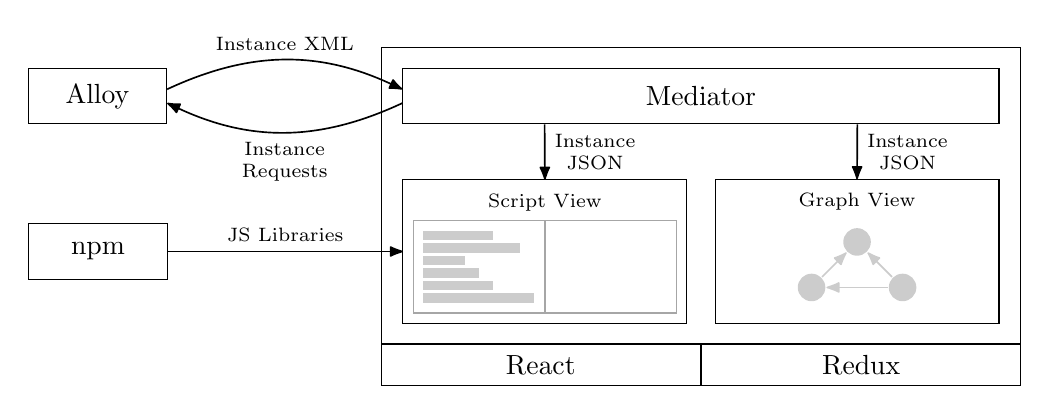
\begin{tikzpicture}[
    tbox/.style={draw, inner sep=0.35em},
    ltbox/.style={draw=black!35, inner sep=0.35em},
    rbox/.style={draw, inner sep=0, minimum width=5em, minimum height=2em},
    dedge/.style={->, >={Latex[round]}, semithick, draw=black}
]

% Script View
{ [
    local bounding box=scriptview, 
    bline/.style={fill=black!20, inner sep=0, anchor=west, minimum height=0.35em}
  ]
\node[bline, minimum width=2.5em, anchor=west] (l1) {};
\node[bline, minimum width=3.5em, below=0.45em of l1.west, anchor=west] (l2) {};
\node[bline, minimum width=1.5em, below=0.45em of l2.west, anchor=west] (l3) {};
\node[bline, minimum width=2em,   below=0.45em of l3.west, anchor=west] (l4) {};
\node[bline, minimum width=2.5em, below=0.45em of l4.west, anchor=west] (l5) {};
\node[bline, minimum width=4em,   below=0.45em of l5.west, anchor=west] (l6) {};
% \node[bline, minimum width=1em,   below=0.45em of l6.west, anchor=west] (l7) {};
% \node[bline, minimum width=3.5em, below=0.45em of l7.west, anchor=west] (l8) {};
\node[ltbox, fit=(l1)(l2)(l3)(l4)(l5)(l6), inner sep=0.35em] (ed) {};
\node[ltbox, fit=(l1)(l2)(l3)(l4)(l5)(l6), inner sep=0.35em, right=0 of ed.east] (vis) {};
\node[above=0.15em of ed.north east, inner sep=0.15em] (sv) {\scriptsize Script View};
\node[tbox, fit=(ed)(vis)(sv), inner sep=0.35em] {};
}

% Graph View
{ [
    local bounding box=graphview, 
    gnode/.style={circle,fill=black!20,thick,inner sep=0pt,minimum size=3.5mm},
    gedge/.style={->, >={Latex[round]}, semithick, draw=black!20}
  ]
\node[tbox, fit=(scriptview), inner sep=0, right=1em of scriptview] (gbox) {};
\node[anchor=north, below=0.15em of gbox.north] (glabel) {\scriptsize Graph View};
\node[gnode, below=0.25em of glabel] (a) {};
\node[gnode, below left=1.25em of a] (b) {}
    edge [gedge] (a) {};
\node[gnode, below right=1.25em of a] (c) {}
    edge [gedge] (b) {}
    edge [gedge] (a) {};
}

% All Views
{ [local bounding box=allviews, inner sep=0]
\node[fit=(scriptview)(graphview)] {};
}

% Sterling
{ [
    local bounding box=sterling
  ]
\node[draw,fit=(scriptview.north west)(graphview.north east), anchor=south, above=2em of allviews.north, minimum height=2em, inner sep=0, label={[yshift=-1.7em]Mediator}] (mediator) {};
\draw [dedge] ([xshift=-5.65em]mediator.south) to node[auto] {\scriptsize\shortstack{Instance\\JSON}} (scriptview.north);
\draw [dedge] ([xshift=5.65em]mediator.south) to node[auto] {\scriptsize\shortstack{Instance\\JSON}} (gbox.north);
\node[tbox, inner sep=0.75em, fit=(mediator)(scriptview)(graphview)] {};
}

% npm
\node[rbox, left=8.5em of scriptview.west] (npm) {npm};
\draw [dedge] (npm.east) to [out=0,in=180] node[auto] {\scriptsize JS Libraries} (scriptview);

% Alloy
\node[rbox, left=8.5em of mediator.west] (alloy) {Alloy};
\draw [dedge] 
    ([yshift=0.25em]alloy.east) to [out=25,in=155] 
    node[auto] {\scriptsize Instance XML} 
    ([yshift=0.25em]mediator.west);
\draw [dedge] 
    ([yshift=-0.25em]mediator.west) to [out=205,in=335] 
    node[auto, align=center] {\scriptsize\shortstack{Instance\\Requests}} 
    ([yshift=-0.25em]alloy.east);
    
% web stack
\node[
    fit=(sterling.south west)(sterling.south),
    anchor=north,
    below=0 of sterling.south,
    rectangle split,
    rectangle split horizontal,
    rectangle split parts=2,
    rectangle split draw splits=true,
    rectangle split part align=base,
    minimum height=1.5em,
    inner sep=0,
    outer sep=0,
    % text width=1em,
    draw] (webstack) {\nodepart{one}React\nodepart{two}Redux};
% \node[draw, fit=(sterling.south west)(sterling.south east), anchor=north, below=0.5em of sterling.south, minimum height=2.5em, inner sep=0, outer sep=0] (webstack) {};
% \node[draw, fit=(scriptview.south west)(scriptview.south east), anchor=north, below=0.75em of scriptview.south, minimum height=1.5em, inner sep=0, outer sep=0, label=center:\scriptsize React] (react) {};
% \node[draw, fit=(scriptview.south west)(scriptview.south east), anchor=west, right=1em of react.east, minimum height=1.5em, inner sep=0, outer sep=0, label=center:\scriptsize Redux] (redux) {};

% { [local bounding box=webstack, node distance=0.35em]
%     \node [ltbox] (js) {JS};
%     \node [ltbox, right=of js] (html) {HTML};
%     \node [ltbox, right=of html] (css) {CSS};
%     \node [tbox, fit=(js)(html)(css)] {};
% }
% { [local bounding box=jsstack, node distance=0.35em]
%     \node [ltbox, above=2.45em of js.west, anchor=west] (react) {React};
%     \node [ltbox, right=of react] (redux) {Redux};
%     \node [tbox, fit=(react)(redux)] {};
% }

% Alloy
% \node [draw, left=of webstack] (alloy) {Alloy};

\end{tikzpicture}
\caption{The Sterling Architecture.}
% A mediator pattern keeps the approach data agnostic so that new visualization techniques can be explored independent of the data source.
\label{fig:sterling}
\end{figure}


The Sterling graph view provides all of the same functionality of the Alloy graph view, but is supported by a few key extensions. 
Most notably, graph elements are not restricted to rows; users may freely arrange graphical elements to make the display more readable. 
Furthermore, the layout algorithm is not automatically executed when the projection is changed or a new instance is generated, and so graphical elements remain static as users step through stateful models and generate instances.
% Furthermore, the layout algorithm is not automatically executed when the projection is updated or when a new instance is generated, unless the graphs do not have any elements in common. As such, graphical elements remain static as users step through stateful models and generate instances.

The Sterling script view provides an environment for the rapid development of custom visualizations by bringing together a text editor, a blank canvas, and a JavaScript execution environment, giving the user a basic ``code sandbox'' in which they can create visualizations based on instance data using their favorite JS libraries.
% The Sterling script view provides an environment for the rapid development of custom visualizations by bringing together three components: a text editor, a blank canvas, and a JavaScript execution environment. 
% This combination gives the user a basic ``code sandbox'' in which they can use their favorite JavaScript libraries to create visualizations based on the instance data. 
Within the script view environment, all instance data---the signatures, fields, atoms, and tuples---are exposed as JS variables. 
Additionally, users have direct access to the npm package repository which can be used to add visualization (or any other useful) libraries to the scripting environment.
% This combination enables, for example, a user to bind atoms to SVG circles using the D3 visualization library, and to calculate their positions based on the relationships defined by the tuples.
This combination enables, for example, a user to bind atoms to shapes using the D3 visualization library, and to calculate their positions based on relationships defined by tuples.
We have found this paradigm to be particularly useful for visualizing instances of models with inherent spatial properties.
For example, a planar embedding of an instance from the previously discussed finite element mesh model is shown in Figure~\ref{fig:script}. More custom visualizations created using the script view, including those used with the sparse matrix model, can be found in the interactive demo on the Sterling website.
% We have found this paradigm to be particularly useful for visualizing instances of models with inherent spatial properties, such as the previously discussed mesh and sparse matrix models shown in Figure~\ref{fig:script}.
Scripts written in the editor are executed each time Sterling receives a new instance or the projection is updated. 
As such, users receive the same kind of immediate visual feedback provided by the graph view, with the added benefit of complete control over the visual abstraction used to present the instance.

\begin{figure}
    \centering
    \frame{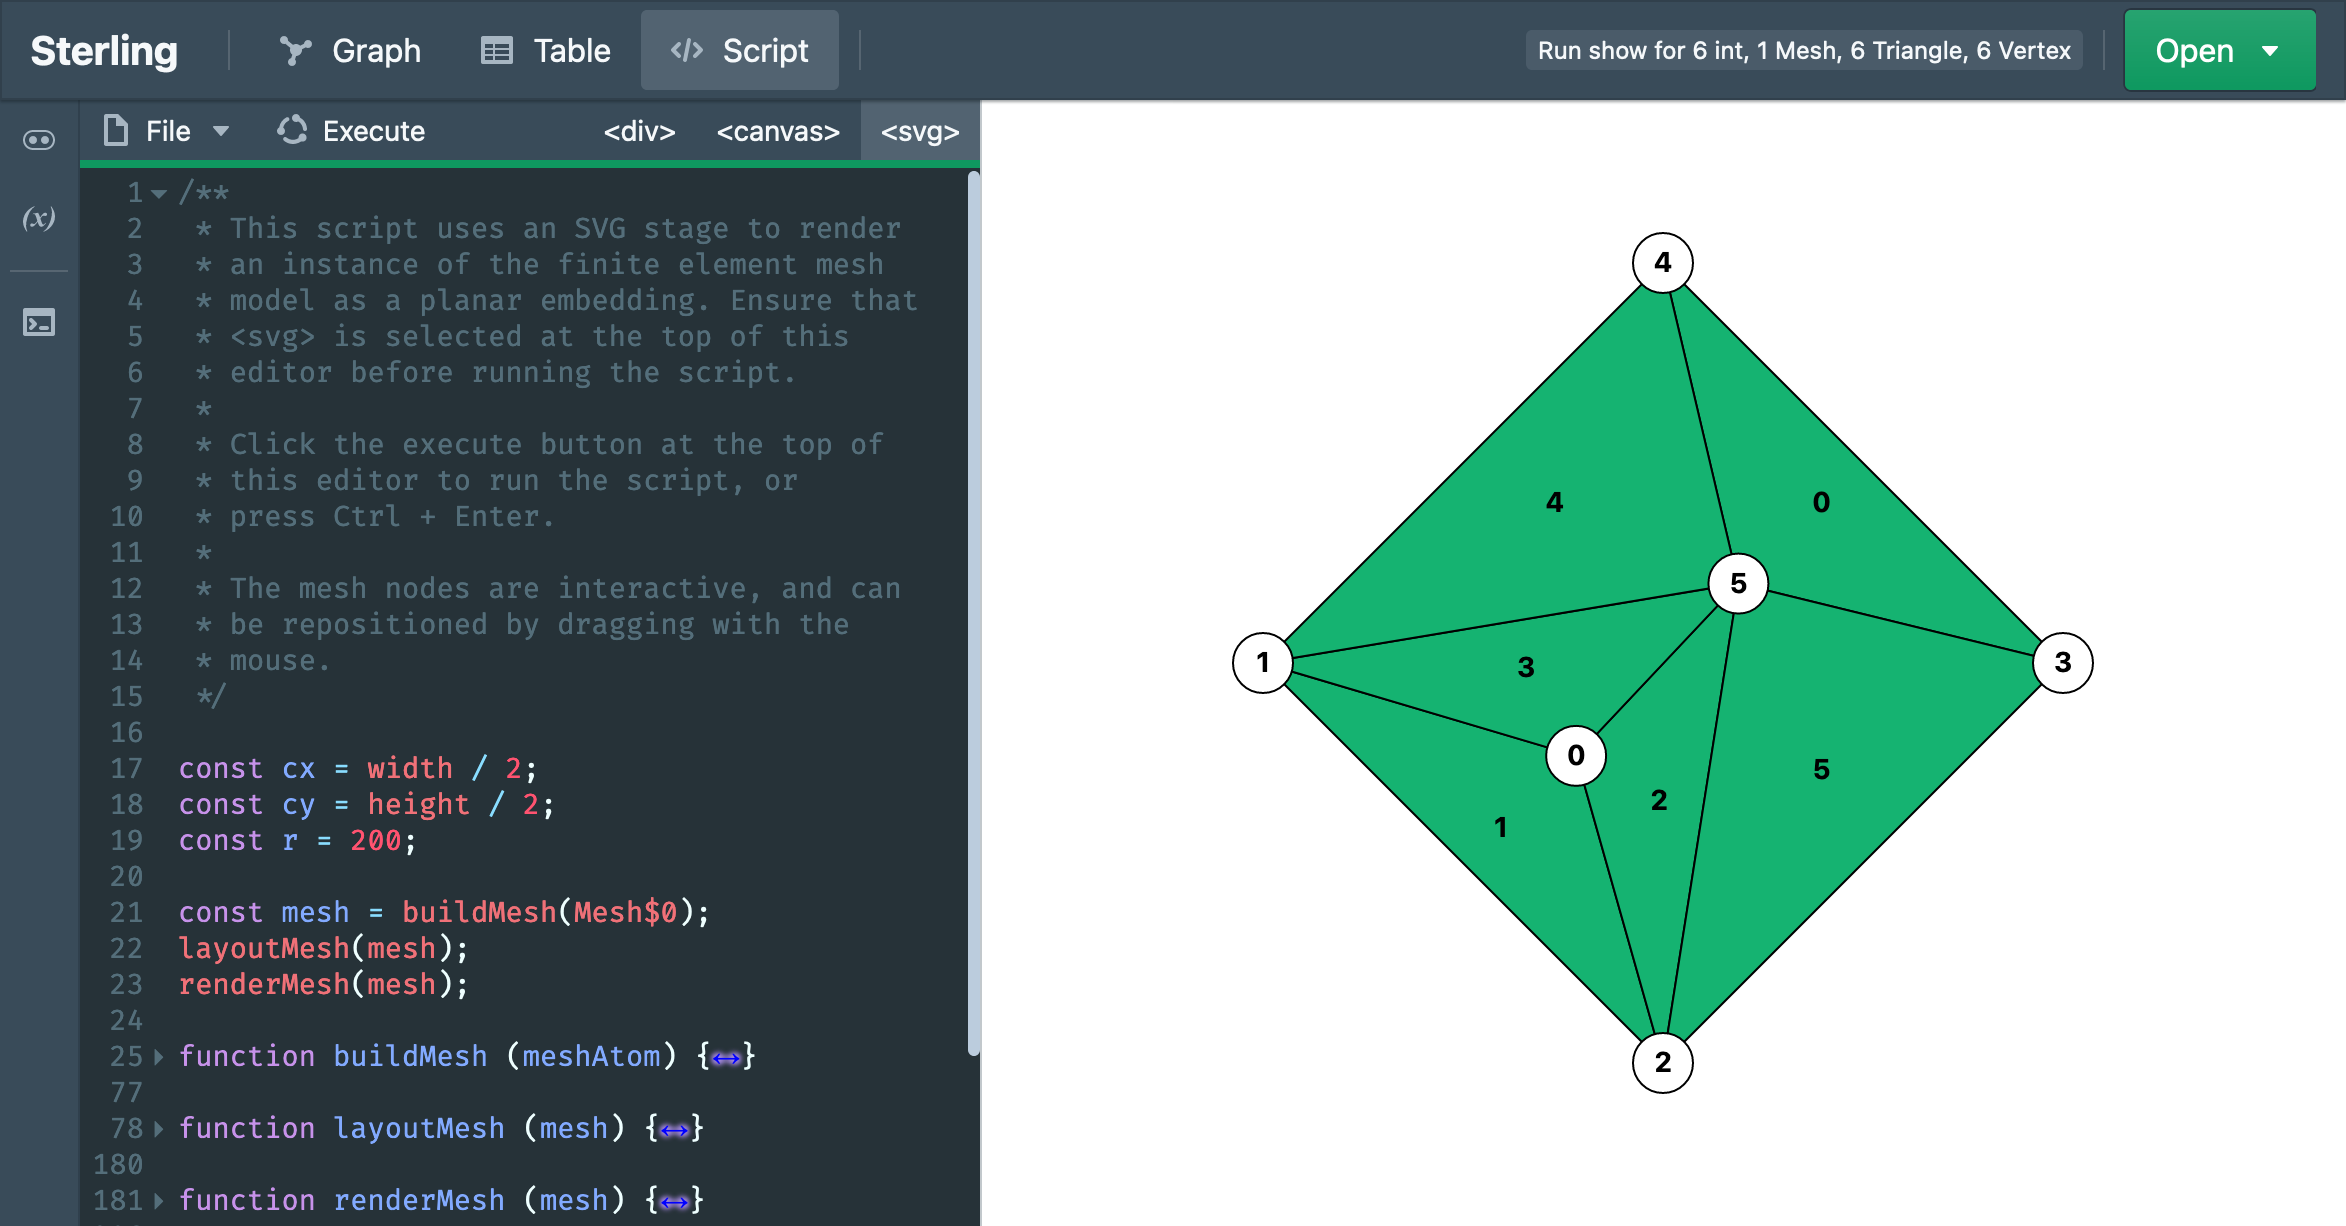
\includegraphics[width=0.95\linewidth]{mesh.png}}
    \caption{An Alloy instance of the finite element mesh model, rendered as a planar embedding in the Sterling script view. Mesh nodes are rendered as white circles and elements as green triangles.}
    % \begin{subfigure}{0.95\textwidth}
    % 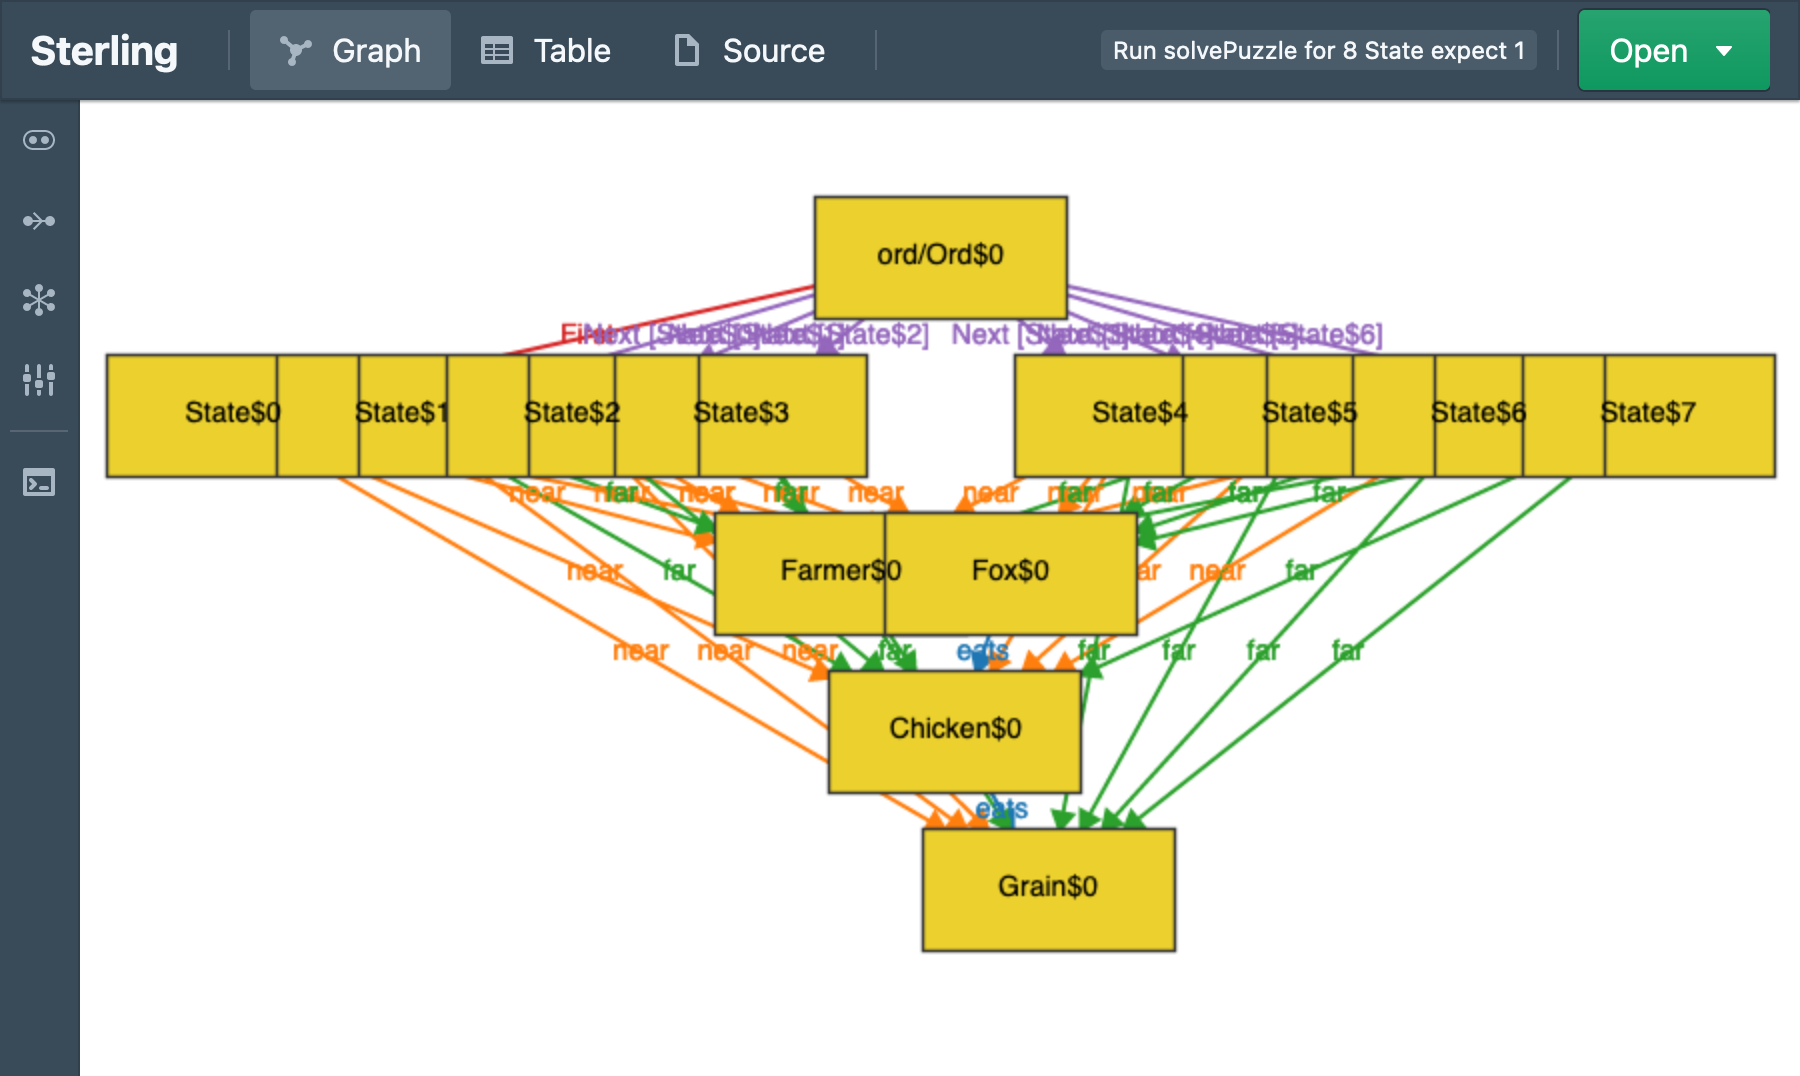
\includegraphics[width=\linewidth]{test.png}
    % \end{subfigure}
    % \caption{Custom visualizations created with the Sterling script view: (1) an instance of the dining philosophers problem in which deadlock has been reached; (2) an instance of a binary tree model in which nodes are positioned based on their presence in the ``left'' and ``right'' relations.}
    \label{fig:script}
\end{figure}

%Sterling is a web application, packaged with a custom build of Alloy, that provides both an enhanced graph visualization to address limitations of Alloy's visualizer and a means for creating custom visualizations when the directed graph representation proves insufficient.
%Drawing on the approach taken by tools like Alloy4Fun~\cite{macedo2019} and BMotionWeb~\cite{ladenberger2016}, a web-based platform was chosen due to the availability of robust data visualization and user interface libraries as well as the popularity of the JavaScript programming language. 
%Consistent with design goals~\ref{dg1} and~\ref{dg2}, Sterling is launched automatically by Alloy when an instance is generated, presenting a familiar user interface. Mirroring the Alloy Visualizer interface, multiple methods for viewing the instance are available through 

\section{Conclusion}
\label{conclusions}
Sterling addresses some of the common issues identified with existing visualizations in Alloy, and introduces a script view to enable development of custom visualizations without sacrificing the immediate visual feedback provided by Alloy as is.
Development is ongoing as part of the lead author's postdoc at Brown University, where Sterling's flexible architecture is being leveraged to develop user studies with the goal of better understanding the role of visualization and user interaction in state-based modeling. 
Additionally, Sterling is the visualizer for an Alloy-like model finder called Forge, developed at Brown University to teach a Logic for Systems class of over 100 students.

% Furthermore, the mediator pattern provides flexibility in terms of data providers and visualizations. 
% Regarding data providers, Alloy need not be the source of data so long as the data being supplied to Sterling adheres to the XML format of an Alloy instance and communication is in adherence with the protocol outlined above. 
% As such, any model finder can be used to supply data for visualization. Indeed, an Alloy-like model finder called Forge, developed at Brown University for a Logic for Systems class, employs Sterling for instance visualization.
% Include a link to the demo!
\bibliographystyle{splncs04}
\bibliography{main}

\end{document}
